\section{Appendix B: Interfaces}

In this section, ways that account data can be imported into the Financial Music software will be explored. An ideal outcome would be that accounts can be imported directly from a website using an API, RSS feed, or other XML based protocol. However, other options will also be considered.

\subsection*{A User Interface}

\label{appendix:interfaces1}The most basic way of having the program attain account information would be to provide a simple user interface.

This interface would consist of fields which can be filled in, and a button to �submit� their contents for analysis.

This kind of interface, whilst crude, would provide a very nice way to test the software. Values could be tweaked and altered on the fly to generate music. Feedback would be instant, providing a quick mental picture of what kind of data produces what kind of music.

\subsection*{Local Sources}

My second reader suggested to me that I use \textbf{CSV} as a commonly used format for importing accounts. This would allow for the easy importing of accounts stored in spreadsheet format (figure: \ref{fig:import1}).

The system I have implemented requires that two year�s worth of accounts be set up in individual spreadsheets. These spreadsheets consist of two rows; the top row contains the headings, and the bottom row contains the numerical values.

The importing procedure runs checks to ensure that both spreadsheets have the same number of columns in the first two rows as each other, and the headings in both spreadsheets are identical. These two clauses provide reasonable assurance that the two spreadsheets are from the same template.

\begin{figure}[ht]
\centering
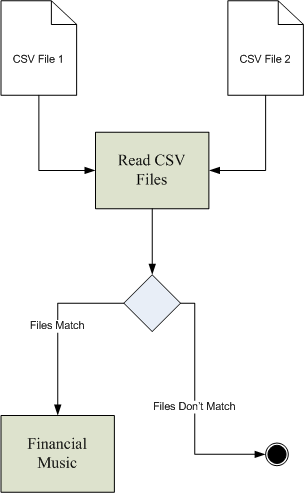
\includegraphics[scale=0.75]{import_1}
\caption{Importing CSV files into the Java application.}
\label{fig:import1}
\end{figure}

\subsection*{Internet Sources}

\label{appendix:interfaces2}The primary candidate for sourcing account information is \textbf{Google Finance}, which has recently launched a localised UK version of this service\footnote{http://finance.google.co.uk, \textit{Google Finance UK}, 01/02/2008}. Google Gadgets provides a JavaScript API for accessing data from Google Finance\footnote{http://code.google.com/apis/gadgets/docs/finance.html, \textit{Financial Gadgets}, 01/02/2008} , but due to licensing restrictions, Google have not opened up this API for use on any other platform\footnote{http://googlefinanceblog.blogspot.com/2007/10/api-gadgets-and-tabs-oh-my.html, 01/02/2008}. \textbf{Yahoo Finance} suffers from a similar restriction, and will only allow the manual generation of HTML as a �badge� that can be placed on a web log (blog) or website\footnote{http://finance.yahoo.com/badges, 01/02/2008}. It also does not provide the complete balance sheet that is needed.

\subsection*{A Workaround}

The option I'm considering is the inclusion of a JavaScript, which can be added as a \textbf{bookmarklet} (a small script or applet stored as a browser bookmark) in a web browser. This JavaScript would be able to scan a web page for specific elements (known as \textbf{data scraping}), and extract them (figure: \ref{fig:import2}). This can be done by accessing elements of the \textbf{document object model} (\textbf{DOM}). Then, the user views a company�s account on Google Finance. They then select the bookmarklet, which runs the JavaScript. The JavaScript could pass the relevant data to another page containing \textbf{Financial Music} as a Java applet\footnote{http://www.devdaily.com/java/edu/pj/pj010003/pj010003.shtml, 01/02/2008}. This would allow an account to be played with a single click. (The idea of disguising a JavaScript as a bookmark is not a new one, as it is used by Google to automate the adding of RSS feeds to Google Reader, and also by \textit{tinyurl.com} to minimise the URL of the currently viewed web page)

There are limitations to this compromise: \textit{(a)} This is all be dependent on Google not changing the setup of their web pages; otherwise the script may no longer function. \textit{(b)} The account information to be extracted is chosen by the JavaScript. Therefore, if we wish to use different account attributes, we need to alter both the JavaScript and the Java Applet to be synchronised with each other.

\begin{figure}[ht]
\centering
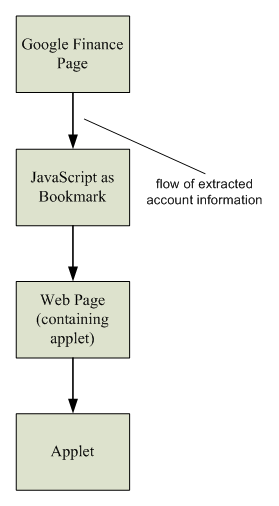
\includegraphics[scale=0.75]{import_2}
\caption{Flow of account data from Google Finance to the Java applet.}
\label{fig:import2}
\end{figure}

\subsection*{In Practice}

The reality of the situation, is that Google Finance isn't set up for easy data extraction (in an ideal situation, the relevant HTML elements would be nicely tagged with the \textit{ID} element). What we do know from looking at the HTML source, is that the value for an attribute is located directly after its label. Therefore, we need to search for the name of the account attribute we want to extract. Once this is done, the next item of data should be the value that we need to extract.

The Java applet should also have a default state, whereby if no information is passed to it via its containing web page, it will allow the user to enter account information manually.